\documentclass{article}

\usepackage[T1]{fontenc} % Umożliwia korzystanie z fontów o kodowaniu T1, które obsługują znaki specjalne używane w językach europejskich.
\usepackage[polish]{babel} % Dostosowuje formatowanie dokumentu do zasad języka polskiego (np. łamanie wierszy, tytuły sekcji).
\usepackage[utf8]{inputenc} % Umożliwia korzystanie z kodowania UTF-8, które obsługuje znaki specjalne i diakrytyczne.
\usepackage{graphicx} % Umożliwia wstawianie obrazów do dokumentu.
\usepackage{subcaption} % Umożliwia tworzenie podpisów dla podobrazów.
\usepackage[margin=2cm]{geometry} % Umożliwia dostosowanie marginesów dokumentu.
\usepackage{listings} % Umożliwia wstawianie kodu źródłowego do dokumentu z odpowiednim formatowaniem.
\usepackage{color} % Umożliwia korzystanie z kolorów w dokumencie.
\usepackage{amsmath} % Rozszerza możliwości formatowania równań matematycznych.
\usepackage{xcolor} % Umożliwia tworzenie kolorowych ram dookoła tekstu.
\usepackage{systeme} % Umożliwia tworzenie systemów równań.
\usepackage{indentfirst} % Powoduje, że pierwszy akapit po tytule sekcji jest wcięty.
\usepackage{dsfont} % Umożliwia korzystanie z dodatkowych fontów, np. dla oznaczeń zbiorów liczbowych.
\usepackage{etoolbox} % Pozwala modyfikować pakiety UŻYWAĆ OSTROŻNIE
\usepackage{blindtext} % Pozwala automatycznie pisać blok lorem ipsum
\usepackage{fancyhdr} % Pozwala na stopki u góry i na dole strony
\usepackage{hyperref} % Umożliwia używanie hyperlinków
\usepackage[justification=centering]{caption}
\hypersetup{
  colorlinks = true,
  linkcolor = black,
  urlcolor = blue,
  pdftitle = {Sprawozdanie z Laboratorium 6} 
}
\patchcmd{\section}{\thispagestyle{plain}}{\thispagestyle{fancy}}{}{}

\definecolor{red}{RGB}{245, 63, 60}
\definecolor{blue}{RGB}{59, 69, 245}
\definecolor{green}{RGB}{72, 225, 17}
\definecolor{yellow}{RGB}{245, 207, 59}

\begin{document}
  \pagestyle{fancy} % pozwala korzystać z pakietu fancyhdr
  \fancyhf{} % clear existing header/footer entries
  \fancyfoot[C]{\thepage}
  \renewcommand{\headrulewidth}{0pt} % Usuń linię na górze strony
  \renewcommand{\footrulewidth}{0.4pt} % Dodaj linię na dole strony  
  \addtolength{\footskip}{0cm} % Zmienia pozycję linii w stopce

  \title{Elektronika Cyfrowa \\ {\large Sprawozdanie z Laboratorium 6}}
  \date{29.05.2024}
  \author{Tomasz Dziób\\{\small Grupa 15}}
  \maketitle

  % Ustawienie Spisu treści do paragrafów 
  \setcounter{tocdepth}{4} % Uwzględnij do typu \paragraph in Spisie treści
  \setcounter{secnumdepth}{4} % Numerowanie do typu \paragraph
  \small \tableofcontents
  \pagebreak

  \section{Wstęp teoretyczny}
    \subsection{Komparator napięcia}
      Jest to układ kombinacyjny służący do porównywania dwóch poziomów napięć. Na wyjściu podaje sygnał zależny od tego, który z sygnałów wejściowych jest większy. Komparator posiada dwa analogowe wejścia $V_{+}$ i $V_{-}$ oraz $V_{0}$. Sygnał wyjściowy idealnego komparatora wynosi: \\

      \begin{figure}[!ht]
        \begin{minipage}{.45\textwidth}
          \begin{equation}
            V_{\mathrm {o} }={\begin{cases}1,&{\mbox{gdy }}V_{+}>V_{-}\\0,&{\mbox{gdy }}V_{+}<V_{-}\end{cases}}
          \end{equation}
        \end{minipage}
        \begin{minipage}{.5\textwidth}
          \centering
          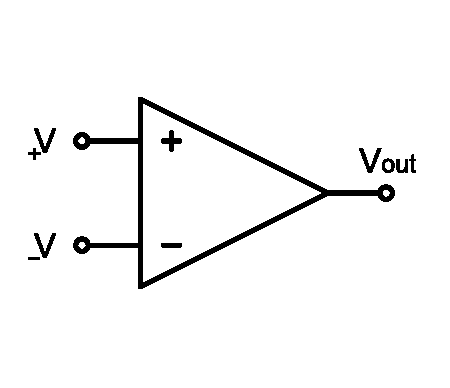
\includegraphics[scale=0.35]{grafiki/Comparator_symbol.eps}
          \caption{Symbol używany do oznaczania komparatora w schematach,
          \\Źródło: \href{https://upload.wikimedia.org/wikipedia/commons/1/1a/Comparator_symbol.svg}{Wikipedia}}
        \end{minipage}
      \end{figure}

    \subsection{Przetwornik C/A}
      Przetwornik C/A (Cyfrowo-Analogowy), znany także jako DAC (Digital-to-Analog Converter), to urządzenie lub układ elektroniczny, który przekształca dane cyfrowe (ciąg bitów) na sygnał analogowy. Umożliwiają wymianę informacji między
      urządzeniami pomiarowymi różnych typów i systemami komputerowymi przetworniki te stanowią łącznik między światem urządzeń analogowych a nowoczesnymi rozwiązaniami cyfrowymi. Znajdują szerokie zastosowania począwszy od domowych multimediów aż po ośrodki naukowe.
      \begin{figure}[!ht]
        \centering
        \includegraphics[scale=0.07]{grafiki/przetwornikCA_zdj.png}
        \caption{Przetwornik CA wykorzystany podczas zajęć,
        \\Źródło: Opracowanie własne}
      \end{figure}
 
    \subsection{Przetwornik A/C typu FLASH}
    jest jednym z najszybszych dostępnych przetworników A/C (Analogowo-Cyfrowy). Jest używany tam, gdzie wymagane są bardzo wysokie prędkości konwersji sygnału analogowego na cyfrowy, na przykład w aplikacjach takich jak cyfrowa obróbka sygnałów, radary, oscyloskopy cyfrowe oraz szybkie transmisje danych.


    Przetworniki A/C stosuje się do przetwarzania napięć stałych, jak również napięć
    zmieniających się w czasie. Pobieranie i przetwarzanie próbek napięcia odbywa się w zadanych chwilach czasu, na ogół okresowo z pewną częstotliwością, zwaną częstotliwością próbkowania. 
    \begin{figure}[!ht]
      \centering
      \includegraphics[scale=0.07]{grafiki/przetwornikAC_zdj.png}
      \caption{Moduł komparatorów wykorzystany w przetworniku A/C typu FLASH zbudowanym podczas zajęć,
      \\Źródło: Opracowanie własne}
      \label{fig1:komparator}
    \end{figure}
    \pagebreak

    \subsection{Transkoder RPP-S (Ręcznie Programowana Pamięć Stała)}
      To urządzenie lub układ elektroniczny wykorzystywany do konwersji danych lub sygnałów między różnymi formatami, przy użyciu ręcznie programowanej pamięci stałej. RPP-S jest specjalnym typem pamięci stałej, która jest zaprogramowana ręcznie, zwykle za pomocą zewnętrznego programatora.
      \begin{figure}[!ht]
        \centering
        \includegraphics[scale=0.07]{grafiki/TranskoderStala_zdj.png}
        \caption{Transkoder RPP-S wykorzystany podczas zajęć,
        \\Źródło: Opracowanie własne}
      \end{figure}

    \subsection{Transkoder PP-SRAN (Ręcznie Programowana Pamięć SRAM)}
      Jest to układ elektroniczny, który wykorzystuje pamięć SRAM (Static Random-Access Memory) do przechowywania danych lub konwersji sygnałów. W przeciwieństwie do pamięci stałej, SRAM jest pamięcią ulotną, co oznacza, że przechowywane w niej dane są tracone po wyłączeniu zasilania. W kontekście transkodera PP-SRAN, ręczne programowanie oznacza, że użytkownik wprowadza dane bezpośrednio do pamięci SRAM.
      \begin{figure}[!ht]
        \centering
        \includegraphics[scale=0.07]{grafiki/TranskoderSRAM_zdj.png}
        \caption{Transkoder PP-SRAN wykorzystany podczas zajęć,
        \\Źródło: Opracowanie własne}
      \end{figure}

  \section{Ćwiczenia}
    \subsection{Ćwiczenie 6.1}
      \subsubsection{Komparator napięcia}
        Pierwsze zadanie dotyczyło stworzenia najprostrzej wersji "układu zmieniającego sygnał analogowy na cyfrowy". Należało użyć płytki UA-1 z komparatorem LM311. Do kontrolowania efektu używany był potencjometr (regulowany dzielnik napięcia).

        \begin{figure}[!ht]
          \begin{minipage}{.5\textwidth}
            \centering
            \includegraphics[scale=0.05]{grafiki/komparator_uklad.jpg}
            \caption{Poprawnie zmontowany układ z komparatorem,
            \\Źródło: Opracowanie własne}
          \end{minipage}
          \begin{minipage}{.5\textwidth}
            \centering
            \includegraphics[scale=0.35]{grafiki/schemat_komparator.jpg}
            \caption{Schemat według którego miało zostać wykonane zadanie pierwsze,
            \\Źródło: \href{https://spe.if.uj.edu.pl/instrukcje}{Strona wykładów}}
          \end{minipage}
        \end{figure}
        Został zbadany przebieg napięcia wyjściowego komparatora dla różnych 
        kształtów napięć i częstotliwości generatora. Przykładowe dwa znajdują się poniżej, reszta w sekcji \textit{Notatki z zajęć}. Kanał pierwszy ukazuje sygnał stworzony przez generator a kanał drugi, reakcję układu.
        \pagebreak
        \begin{figure}[!ht]
          \begin{minipage}{.5\textwidth}
            \centering
            \includegraphics[scale=0.35]{grafiki/komparator_2.5kHz_15V_ramp.png}
            \caption{Reakcja zbudowanego układu na sygnał trójkątny ($2,5kHz$ i $15V$),
            \\Źródło: Opracowanie własne}
          \end{minipage}
          \begin{minipage}{.5\textwidth}
            \centering
            \includegraphics[scale=0.35]{grafiki/komparator_5kHz_10V_sin.png}
            \caption{Reakcja zbudowanego układu na sygnał sinusoidalny ($5kHz$ i $10V$),
            \\Źródło: \href{https://spe.if.uj.edu.pl/instrukcje}{Strona wykładów}}
          \end{minipage}
        \end{figure}

        Zmiana pokrętła potencjometru wiąże się ze zmniejszeniem amplitudy. Dla oporu wynoszącego $0Ohm$ uzyskujemy linię prostą.

        \begin{figure}[!ht]
          \centering
          \includegraphics[scale=0.3]{grafiki/komparator_5kHz_10V_sin_0ohm.png}
          \caption{Reakcja zbudowanego układu na sygnał sinusoidalny ($5kHz$ i $10V$) przy potencjometrze ustawionym na $0Ohm$,
          \\Źródło: Opracowanie własne}
        \end{figure}


      \subsubsection{Wzmacniacz operacyjny}
        W ten sam sposób został przetestowany układ zawierający wzmacniacz operacyjny zamiast komparatora.

        \begin{figure}[!ht]
          \begin{minipage}{.5\textwidth}
            \centering
            \includegraphics[scale=0.3]{grafiki/wzmacniacz_1kHz_10V_ramp_10kOhm.png}
            \caption{Reakcja układu ze wzmacniaczem na sygnał trójkątny ($1kHz$ i $10V$),
            \\Źródło: Opracowanie własne}
          \end{minipage}
          \begin{minipage}{.5\textwidth}
            \centering
            \includegraphics[scale=0.3]{grafiki/wzmacniacz_1kHz_10V_sin_10kOhm.png}
            \caption{Reakcja układu ze wzmacniaczem na sygnał sinusoidalny ($1kHz$ i $10V$),
            \\Źródło: Opracowanie własne}
          \end{minipage}
        \end{figure}

        Dla wyższych częstotliwości można było zauważyć odstępstwa od wcześniejszych przebiegów (patrz Rysunek 13).

        \begin{figure}[!ht]
          \begin{minipage}{.5\textwidth}
            \centering
            \includegraphics[scale=0.3]{grafiki/wzmacniacz_10kHz_10V_sin_10kOhm.png}
            \caption{Reakcja układu ze wzmacniaczem na sygnał trójkątny ($10kHz$ i $10V$) różniąca się przebiegiem od reszty,
            \\Źródło: Opracowanie własne}
          \end{minipage}
          \begin{minipage}{.5\textwidth}
            \centering
            \includegraphics[scale=0.06]{grafiki/wzmacniacz_zdj.png}
            \caption{Poprawnie zmontowany układ ze wzmacniaczem,
            \\Źródło: Opracowanie własne}
          \end{minipage}
        \end{figure}

        Poniżej zamieszczam film prezentujący działanie układu (z podłączonym komparatorem) \href{https://youtu.be/iaurY3viG4w}{[LINK]}.

    \subsection{Ćwiczenie 6.2}
      Zadanie drugie dotyczyło zmontowania przetwornika C/A. Został on zbudowany z sumatora napięć oraz licznika modulo 8 których implementacje budowaliśmy na poprzednich zajęciach. W celu uzyskania działającego układu należało wejścia z licznika podłączyć według poniższego schematu.

      \begin{figure}[!ht]
        \centering
        \includegraphics[scale=0.45]{grafiki/6.2_schemat.jpg}
        \caption{Schemat przetwornika C/A wykorzystany w tym zadaniu,
        \\Źródło: \href{https://spe.if.uj.edu.pl/instrukcje}{Strona wykładów}}
      \end{figure}

      $U_1$, $U_2$,$U_3$ oznaczają wejścia licznika z podpiętymi dopowiednio opornikami.Wykorzystując podstawowe prawa łączenia oporników można ten zapis uprościć do $R = R_2, R_1 = \frac{R_2}{2}, R_3 = 2 \cdot R_2$. Dzięki temu można zdefiniować jakie wartości oporników zostały użyte podczas budowy układu: \\
      $R_1 = 1,489 k \Omega$ \\
      $R_2 = 2,969 k \Omega$ \\
      $R_3 = 6,09 k \Omega$ \\
      Na licznik została wpuszczona fala prostokątna z generatora.
      \begin{figure}[!ht]
        \begin{minipage}{.5\textwidth}
          \centering
          \includegraphics[scale=0.06]{grafiki/6.2_zdj.jpg}
          \caption{Poprawnie zbudowany Przetwornik C/A przy pomocy licznika modulo 8 oraz sumatora napięć,
          \\Źródło: Opracowanie własne}
        \end{minipage}
        \begin{minipage}{.5\textwidth}
          \centering
          \includegraphics[scale=0.35]{grafiki/schodki.png}
          \caption{Odczyt z oscyloskopu prezentowanego obok układu --- zdigitalizowany sygnał analogowy do postaci widocznych rozróżnialnych stanów,
          \\Źródło: Opracowanie własne}
        \end{minipage}
      \end{figure}
      \pagebreak
      
    \subsection{Ćwiczenie 6.3}
      Jest to zadanie praktycznie dopiero rozpoczynające ćwiczenia jednak nie w tym przypadku. Z powodu braku czaso zostało ono jedynie napoczęte. Polegało na zapoznaniu się z budową i działaniem modułów przetwornika A/C typu FLASH takimi jak modułem komparatorów, transkoderem RPP-S (Ręcznie Programowana Pamięć Stała) oraz transkoderem RPP-SRAN (Ręcznie Programowana Pamięć SRAM).

      \begin{figure}[!ht]
        \begin{minipage}{.5\textwidth}
          \centering
          \includegraphics[scale=0.07]{grafiki/6.3_zdj.png}
          \caption{Układ który udało się zbudować podczas wykonywania tego zadania (z racji niepełnego przebadania jego działania nie jestem wstanie stwierdzić czy jest on poprawny),
          \\Źródło: Opracowanie własne}
        \end{minipage}
        \begin{minipage}{.5\textwidth}
          \centering
          \includegraphics[scale=0.35]{grafiki/przetwornik_A_C.png}
          \caption{Odczyt z oscyloskopu który udało się zapisać po złączeniu wszystkich segementów. Widać w małym stopniu dygitalizację sygnału,
          \\Źródło: Opracowanie własne}
        \end{minipage}
      \end{figure}

      Układ został zbudowany oraz podłączony do generatora. Pozwoliło to na powieszchowne zbadanie układu. Udało się uzyskać prosta rekację układu na sygnał sinusoidalny z generatora. Była to wizualizacja napięcia na diodach układu (\ref{fig1:komparator}) \href{https://youtu.be/hi4uA4t9sUA}{[LINK DO NAGRANIA]}. Wraz ze zmniejszeniem napięcia zaobserwować można było mniej diod świecących się w rytm przebiegu funkcji sinus do modułu.
      

  \section{Omówienie wyników}
    \subsection{Ćwiczenie 6.1}
      Zadanie przebiegło po myśli, udało się zbudować dwie, poprawnie działające, wersje układu. Zmiana oporu na potencjometrze powodowała spadek amplitudy aż do uzyskania przebiegu liniowego (dla całkowtego braku oporu).
    \subsection{Ćwiczenie 6.2}
      Było to zadanie które pochłonęło zdecydowanie za dużą część tych ćwiczeń. Polegało na zbudowaniu dwóch osobnych układów, licznika modulo 8 i sumatora napięć. Licznik został podłączony na początku, oraz przebadany na wskaźnikach LED na płytce. Z sukcesem przechodził on przez wszystkie stany tego układu nie wskazując na błędną budowę, więc rozpoczęto prace nad drugim układem. Z racji, że wymagał on dobrania odpowiednich oporników, ich wybór cały czas był podważany. Spowodowane to było nieregularnym przebiegiem układu odczytywanym z oscyloskopu. Łącznie zestawy różnych oporników były wymieniane 3-krotnie. Następnie podejrzenie padło na użyte kable oraz wadliwą płytkę. Żadna zmiana jednak nie zmieniła nic w przebiegu. 
      
      Koniem trojańskim układu okazał się licznik który mimo poprawnego działania powodował błędne odczyty. Opierając jego budowę na implementacji z poprzednich zajęć (licznik modulo 10) z rozpędu podłączyłem dodatkowy moduł licznika tworząc najpierw wersję modulo 16 aby później ``ograniczyć'' ją do modulo 8. Dało się to jednak stworzyć prościej korzystając tylko z podstawowych 3 modułów. Było to przyczyną wadliwych przebiegów układu. Na papierze ta sama funkcja --- w rzeczywistości powodowała błędy.


      \begin{figure}[!ht]
        \centering
        \includegraphics[scale=0.5]{grafiki/7493_01.png}
          \caption{Wewnętrzna sieć logiczna licznika 7493 wykorzystanego w tym zadaniu -- widać poszczególne moduły A, B, C i D,
          \\Źródło: \href{https://eduinf.waw.pl/inf/prg/010_uc/7493.php}{7493 – 4-bitowy licznik dwójkowy (moduły 2 i 8)}}
      \end{figure}

    \subsection{Ćwiczenie 6.3}
      Budowa układu z tego ćwiczenia przebiegła według oczekiwań. Całość po podłączeniu zadziałała oraz wstępnie wizualizowała zmieniane napięcie amplitudy funkcji. Niestety nic więcej nie udało się zaobserwować ze względu na czas zakończenia zajęć.

  \section{Podsumowanie}
    Laboratorium numer 6 polegało na zbudowaniu układów elektronicznych, które miały na celu przetwarzanie sygnałów analogowych na cyfrowe oraz odwrotnie. Stworzone zostały: układ z komparatorem napięcia oraz wzmacniaczem operacyjnym, które pozwoliły na przekształcenie różnych sygnałów wejściowych,   
    przetwornik cyfrowo-analogowy (C/A). Zbudowanie układu z sumatorem napięć oraz licznikiem modulo 8 czy moduł przetwornika A/C typu FLASH.

    Podsumowując, laboratorium było czasochłonne i pozwoliło na zdobycie praktycznej wiedzy z zakresu elektroniki cyfrowej, przetwarzania sygnałów oraz budowy układów cyfrowo-analogowych. Napotkane problemy były cennymi lekcjami, które przyczynią się do lepszego zrozumienia zasady działania omawianych komponentów i układów.
    
  \section{Notatki z zajęć}
  
  \begin{figure}[!ht]
    \begin{minipage}{.5\textwidth}
      \centering
      \includegraphics[scale=0.12]{grafiki/notatki.jpg}
      \caption{Notatki wykonane w czasie zajęć,
      \\Źródło: Opracowanie własne}
    \end{minipage}
    \begin{minipage}{.5\textwidth}
      \centering
      \includegraphics[scale=0.06]{grafiki/notatki2.jpg}
      \caption{Notatki wykonane w czasie zajęć,
      \\Źródło: Opracowanie własne}
    \end{minipage}
  \end{figure}

  \begin{figure}[!ht]
    \begin{minipage}{.5\textwidth}
      \centering
      \includegraphics[scale=0.06]{grafiki/reakcja2.jpg}
      \caption{Reakcja układu na pozycję potencjometru,
      \\Źródło: Opracowanie własne}
    \end{minipage}
    \begin{minipage}{.5\textwidth}
      \centering
      \includegraphics[scale=0.06]{grafiki/reakcja1.jpg}
      \caption{Reakcja układu na pozycję potencjometru,
      \\Źródło: Opracowanie własne}
    \end{minipage}
  \end{figure}

  \begin{figure}[!ht]
    \begin{minipage}{.5\textwidth}
      \centering
      \includegraphics[scale=0.35]{grafiki/komparator_100kHz_10V_sin.png}
      \caption{Odczyt z układu z komparatorem dla $100kHz$ $10V$ fali sinusoidalnej,
      \\Źródło: Opracowanie własne}
    \end{minipage}
    \begin{minipage}{.5\textwidth}
      \centering
      \includegraphics[scale=0.35]{grafiki/wzmacniacz_1kHz_10V_sin_0Ohm.png}
      \caption{Odczyt z układu ze wzmacniaczem dla $1kHz$ $10V$ fali sinusoidalnej oraz oporu $0Ohm$,
      \\Źródło: Opracowanie własne}
    \end{minipage}
  \end{figure}

  \begin{figure}[!ht]
    \centering
    \includegraphics[scale=0.35]{grafiki/wzmacniacz_30kHz_10V_ramp_10kOhm.png}
      \caption{Odczyt z układu ze wzmacniaczem dla $30kHz$ $10V$ fali trójkątnej oraz oporu $10kOhm$,
      \\Źródło: Opracowanie własne}
  \end{figure}

\end{document}